%\documentclass[prb,aps,nobibnotes,twocolumn,doublespace,twocolumngrid,superbib]{revtex4}
\documentclass[prb,aps,nobibnotes,superbib,preprint]{revtex4}

\usepackage{graphicx}
\usepackage{amsfonts}
\usepackage{amsmath}
\usepackage{bm}
\usepackage{alltt}
\usepackage{dcolumn} 
\usepackage{graphicx}
\makeatletter 
\makeatother

\begin{document}

\title{\textbf{Exact Bounded Multipole Error Estimates for O(N) Tree Codes}}

\author{C. J. Tymczak}
\author{Matt Challacombe}

\affiliation{Theoretical Division, Los Alamos National Laboratory, Los Alamos,NM 87545, USA}

\date{\today}

\begin{abstract}
Periodic boundary conditions have been implemented in the linear scaling
Quantum Chemistry code \textbf{MondoSCF}.
\end{abstract}


\maketitle

\section{Introduction}

\section{Scaling}


\section{CONCLUSIONS}


\section*{ACKNOWLEDGMENTS}

We would like to acknowledge Tommy Sewell and Ed Kober for there advise
and support. We would also like to thank Anders Niklasson for his help
in preparation of this manuscript. 

\bibliographystyle{apsrmp} 
\bibliography{mondo}


\appendix

\section{Exact Error Bound for the MAC}
Let us start by defining some useful quantities
\begin{equation}
\label{B1}
\widehat{O}_{l}^{m}\left[ \mathbf{R}\right] =\frac{\left| \mathbf{R}\right| ^{l}P_{l}^{m}
\left( \cos \theta _{\mathbf{R}}
\right) \, e^{-im\phi _{\mathbf{R}}}}{\left( l+m\right) !}\quad \; \; 
\end{equation}
\begin{equation}
\label{B2}
M_{l}^{m}\left[ \mathbf{R}\right] =\frac{\left( l-m\right) !\, P_{l}^{m}\left( \cos 
\theta _{\mathbf{R}}\right) \, 
e^{-im\phi _{\mathbf{R}}}}{\left| \mathbf{R}\right| ^{l+1}}
\end{equation}
\begin{equation}
\label{B3}
{\cal O}_{l}^{m}\left[ \rho ;\mathbf{P}\right] =\int _{V_{\infty }}\, d{\mathbf{r}}\, 
\widehat{O}_{l}^{m}\left[ 
{\mathbf{r}-\mathbf{P}}\right] \, \rho \left( \mathbf{r}\right) \qquad \; \; \; 
\end{equation}
Next, let us consider the expansion of the coulomb integral into the
multipole basis\[
\int \, d{\mathbf{r}}\, d{\mathbf{r}'}\frac{\rho _{1}\left( \mathbf{r}\right) \: \rho _{2}
\left( \mathbf{r}'\right) }
{\left| \mathbf{r}-\mathbf{r}'\right| }\qquad \qquad \qquad \qquad \qquad \qquad \qquad 
\qquad \qquad \qquad \qquad 
\qquad \qquad \]
\begin{equation}
\label{B4}
\approx \frac{1}{2}\sum _{l=0}^{L}\, \sum _{l'=0}^{L'}\, \sum _{m=-l}^{l}\, \sum _{m'=-l'}^{l'}\,
 \left( -1\right) ^{l}
\, {\cal O}_{l}^{m}[\rho _{1};\mathbf{P}]M_{l+l'}^{m+m'}[\mathbf{P}-\mathbf{Q}]\, 
{\cal O}_{l'}^{m'}[\rho _{2};\mathbf{Q}]
\end{equation}
Let us now assume that the primitive distribution \( \rho _{1} \)
is of a single angular momentum type and expanded about its center, 

\begin{equation}
\label{B5}
{\cal O}_{l}^{m}[\rho _{1};\mathbf{P}]={\cal O}_{l}^{m}[\rho _{1};\mathbf{P}]\delta _{l\, l_{0}}
\end{equation}
this gives us\[
\int \, d{\mathbf{r}}\, d{\mathbf{r}'}\frac{\rho _{1}\left( \mathbf{r}\right) \: \rho _{2}
\left( \mathbf{r}'\right) }
{\left| \mathbf{r}-\mathbf{r}'\right| }\qquad \qquad \qquad \qquad \qquad \qquad \qquad 
\qquad \qquad \qquad \qquad 
\qquad \qquad \]
\begin{equation}
\label{B6}
\approx \frac{1}{2}\sum _{l'=0}^{L'}\, \sum _{m=-l_{0}}^{l_{0}}\, \sum _{m'=-l'}^{l'}\, 
\left( -1\right) ^{l}\, 
{\cal O}_{l_{0}}^{m}[\rho _{1};\mathbf{P}]\, M_{l_{0}+l'}^{m+m'}[{\mathbf{P}-\mathbf{Q}}]\, 
{\cal O}_{l'}^{m'}[\rho _{2};
\mathbf{Q}]
\end{equation}
The error in the calculation is then the multipoles that we do not
sum\begin{equation}
\label{B7}
\varepsilon \left( l_{0}\right) =\left| \frac{1}{2}\sum _{l'=L'+1}^{\infty }\, 
\sum _{m=-l_{0}}^{l_{0}}\, 
\sum _{m'=-l'}^{l'}\, \left( -1\right) ^{l}\, {\cal O}_{l_{0}}^{m}[\rho _{1};\mathbf{P}]\, 
M_{l_{0}+l'}^{m+m'}
[{\mathbf{P}-\mathbf{Q}}]\, {\cal O}_{l'}^{m'}[\rho _{2};\mathbf{Q}]\right| 
\end{equation}
 Let us define for the unsold operator\[
{\cal \widehat{O}}_{l}\left[ \left| \mathbf{P}\right| \right] =\sqrt{\sum _{m}(l-m)!(l+m)!
\left| \widehat{O}_{l}^{m}
\left[ \mathbf{P}\right] \right| ^{2}}\]
\begin{equation}
\label{B8}
\qquad \qquad \qquad \quad =\left| \mathbf{P}\right| ^{l}\sqrt{\sum _{m}\frac{(l-m)!}{(l+m)!}
\left| P_{l}^{m}
(\mathbf{P})\right| ^{2}}=\left| \mathbf{P}\right| ^{l}\geq 0
\end{equation}
and similarly the unsold weights\begin{equation}
\label{B9}
{\cal O}_{l}[\rho ;\left| \mathbf{P}\right| ]=\sqrt{\sum _{m}(l-m)!(l+m)!\left| {\cal O}_{l}^{m}
\left[ \rho ;\left| 
\mathbf{P}\right| \right] \right| ^{2}}
\end{equation}
Let us rewrite the error bound as\begin{equation}
\label{B10}
\varepsilon \left( l_{0}\right) \leq \frac{1}{2}\sum _{l'=L'+1}^{\infty }\left| \, 
\sum _{m=-l_{0}}^{l_{0}}\, 
\sum _{m'=-l'}^{l'}{\cal O}_{l_{0}}^{m}[\rho _{1};\mathbf{P}]\, M_{l_{0}+l'}^{m+m'}
[{\mathbf{P}-\mathbf{Q}}]\, 
{\cal O}_{l'}^{m'}[\rho _{2};\mathbf{Q}]\right| 
\end{equation}
Let us also, for compactness of notation, define 
\begin{equation}
\label{B11}
{\cal O}_{l}^{m}\equiv {\cal O}_{l}^{m}[\rho _{1};\mathbf{P}]
\end{equation}
where the placement will indicate which distribution it is derived
from. Using equations (\ref{B2}) and (\ref{B3}) we can write this
as
\[
\varepsilon \left( l_{0}\right) \leq \frac{1}{2}\sum _{l'=L'+1}^{\infty }\, \left| 
\sum _{m=-l_{0}}^{l_{0}}\, 
\sum _{m'=-l'}^{l'}\frac{(l_{0}+l'-(m+m'))!}{\sqrt{(l_{0}+m)!(l_{0}-m)!}\: \sqrt{(l'+m')!(l'-m')!}}\right. 
\qquad \qquad \]
\begin{equation}
\label{B12}
\qquad \left. \frac{\sqrt{(l_{0}+m)!(l_{0}-m)!}{\cal O}_{l_{0}}^{m}\, P_{l_{0}+l'}^{m+m'}\left( \cos 
\theta _{\mathbf{PQ}}\right) \, \sqrt{(l'+m')!(l'-m')!}{\cal O}_{l'}^{m'}}{\left| \mathbf{P}-\mathbf{Q}
\right| ^{l'+l_{0}+1}}\right| 
\end{equation}
for reasons which will become apparent in what follows. Let us use
the inequalities (ref)\begin{equation}
\label{B13}
\left| P_{l}^{m}\left( \cos \theta _{\mathbf{R}}\right) \right| \leq 1
\end{equation}
to simplify\[
\varepsilon \left( l_{0}\right) \leq \frac{1}{2}\sum _{l'=L'+1}^{\infty }\, \left| 
\sum _{m=-l_{0}}^{l_{0}}\, 
\sum _{m'=-l'}^{l'}\frac{(l_{0}+l'-(m+m'))!}{\sqrt{(l_{0}+m)!(l_{0}-m)!}\: \sqrt{(l'+m')!(l'-m')!}}
\right. \qquad \qquad \]
\begin{equation}
\label{B14}
\qquad \qquad \left. \frac{\sqrt{(l_{0}+m)!(l_{0}-m)!}\, {\cal O}_{l_{0}}^{m}\, 
\sqrt{(l'+m')!(l'-m')!}\, 
{\cal O}_{l'}^{m'}}{\left| \mathbf{P}-\mathbf{Q}\right| ^{l'+l_{0}+1}}\right| 
\end{equation}
 Now, let use the inequality (ref)\[
\left| \mathbf{a}\cdot \mathbf{b}\right| \leq \left| \mathbf{a}\right| \left| \mathbf{b}\right| 
\qquad \qquad \]
\begin{equation}
\label{B15}
\left| \sum _{n}a_{n}\, b_{n}\right| \leq \sqrt{\sum _{n}\left| a_{n}\right| ^{2}\sum _{n'}
\left| b_{n'}\right| ^{2}}
\end{equation}
to get\[
\varepsilon \left( l_{0}\right) \leq \frac{1}{2}\sum _{l'=L'+1}^{\infty }\sqrt{\sum _{m=-l_{0}}^{l_{0}}\, 
\sum _{m'=-l'}^{l'}\frac{\left[ (l_{0}+l'-(m+m'))!\right] ^{2}}{(l_{0}+m)!(l_{0}-m)!\, (l'+m')!(l'-m')!}}
\qquad 
\qquad \qquad \qquad \qquad \]
\begin{equation}
\label{B16}
\frac{\sqrt{\sum ^{l_{0}}_{m''=-l_{0}}\sum _{m'''=-l'}^{l'}(l_{0}+m'')!(l_{0}-m'')!\left| 
{\cal O}_{l_{0}}^{m''}\right|
 ^{2}\: (l'+m''')!(l'-m''')!\left| {\cal O}_{l'}^{m'''}\right| ^{2}}}{\left| \mathbf{P}-\mathbf{Q}
\right| ^{l'+l_{0}+1}}
\end{equation}
Which we can rewrite very compactly as 
\begin{equation}
\label{B17}
\varepsilon \left( l_{0}\right) \leq \frac{1}{2}\sum _{l'=L'+1}^{\infty }\frac{{\cal O}_{l_{0}}
[\rho _{1};\left|
 \mathbf{P}\right| ]\: N\left[ l_{0},l'\right] \: {\cal O}_{l'}[\rho _{2};\left| \mathbf{Q}\right| ]}
{\left| 
\mathbf{P}-\mathbf{Q}\right| ^{l'+l_{0}+1}}
\end{equation}
where\begin{equation}
\label{B18}
N\left[ l,l'\right] =\sqrt{\sum _{m=-l_{0}}^{l_{0}}\, \sum _{m'=-l'}^{l'}\frac{\left[ (l_{0}+l'-(m+m'))!
\right] ^{2}}{(l_{0}+m)!(l_{0}-m)!\, (l'+m')!(l'-m')!}}
\end{equation}
However, we still have to eliminate the infinite sum over \( l' \)
within our error expression. Let us consider the limit of

\begin{equation}
\label{B19}
\lim _{l\rightarrow \infty }\left\{ {\cal O}_{l}[\rho ;\left| \mathbf{P}\right| ]\right\} ^{1/l}
\end{equation}
 Considering the density as a sum of delta functions with arbitrary
weights. 

\begin{equation}
\label{B20}
\rho \left( \mathbf{r}\right) =\sum _{i}c_{i}\, \delta \left( \mathbf{r}-\mathbf{r}_{i}\right) 
\end{equation}
 then for the multipoles\begin{equation}
\label{B21}
{\cal O}_{l}^{m}\left[ \rho ;\mathbf{P}\right] =\int _{V_{\infty }}\, d\mathbf{r}\, 
\widehat{O}_{l}^{m}\left[ 
\mathbf{r}-\mathbf{P}\right] \, \rho \left( \mathbf{r}\right) =\sum _{i}c_{i}\, 
\widehat{O}_{l}^{m}\left[ 
\mathbf{r}_{i}-\mathbf{P}\right] 
\end{equation}
and for the unsold weights\begin{eqnarray*}
{\cal O}_{l}[\rho ;\left| \mathbf{P}\right| ] & = & \sqrt{\sum _{m}(l-m)!(l+m)!\left| 
{\cal O}_{l}^{m}\left[ 
\rho ;\left| \mathbf{P}\right| \right] \right| ^{2}}\\
 & = & \sqrt{\sum _{m}(l-m)!(l+m)!\left| \sum _{i}c_{i}\, \widehat{O}_{l}^{m}\left[ 
\mathbf{r}_{i}-\mathbf{P}
\right] \right| ^{2}}
\end{eqnarray*}
\begin{equation}
\label{B22}
\; 
\end{equation}
which we can rewrite using the addition therom of anglular momentum
as (ref)\begin{equation}
\label{B23}
{\cal O}_{l}[\rho ;\left| \mathbf{P}\right| ]=\sqrt{\sum _{ij}c_{i}\, c_{j}^{*}\, \left| 
\mathbf{r}_{i}-
\mathbf{P}\right| ^{l}\left| \mathbf{r}_{j}-\mathbf{P}\right| ^{l}\, P_{l}\left[ 
\cos \gamma _{ij}\right] }
\end{equation}
which allows us to take the limit\begin{equation}
\label{B24}
\lim _{l\rightarrow \infty }\left\{ {\cal O}_{l}[\rho ;\left| \mathbf{P}\right| ]\right\} ^{1/l}=
\lim _{l\rightarrow 
\infty }\left\{ \left| c_{I}\right| \, \left| \mathbf{d}_{max}\right| ^{l}\right\} ^{1/l}=\left|
 \mathbf{d}_{max}\right| 
\end{equation}
where \( \left| \mathbf{d}_{max}\right|  \)is the maximum distance
of a distribution to the contraction center \( \left| \mathbf{P}\right|  \).
Let us rewrite equation (\ref{B17}) as\begin{equation}
\label{B25}
\varepsilon \left( l_{0}\right) \leq \frac{1}{2}\frac{{\cal O}_{l_{0}}\left[ \rho _{1};\left|
 \mathbf{P}\right| 
\right] }{\left| \mathbf{P}-\mathbf{Q}\right| ^{l_{0}+L'+2}}\sum _{l=0}^{\infty }\frac{N\left[ 
l_{0},l+L'+1\right]
 {\cal O}_{l+L'+1}\left[ \rho _{1};\left| \mathbf{Q}\right| \right] }{\left| \mathbf{P}-\mathbf{Q}
\right| ^{l}}
\end{equation}
Analyzing the behavior of \( N\left[ l,l'\right]  \) for large \( l' \)
we find that\begin{equation}
\label{B26}
N\left[ l,l'\right] \leq \alpha _{l}\frac{\left( \left( 1+l'\right) \left( 2+l'\right) \ldots 
\left( l+l'\right)
 \right) }{l!}=\alpha _{l}\frac{(l+l')!}{l!\, l'!}\equiv n\left[ l,l'\right] 
\end{equation}
where \( \alpha _{l}\leq \sqrt{2} \). Using equation (\ref{B26})
this can be written as\begin{equation}
\label{B27}
\varepsilon \left( l_{0}\right) \leq \frac{1}{2}\frac{{\cal O}_{l_{0}}\left[ \rho _{1};\left| 
\mathbf{P}\right| 
\right] }{\left| \mathbf{P}-\mathbf{Q}\right| ^{l_{0}+L'+2}}\sum _{l=0}^{\infty }\frac{n\left[ 
l_{0},l+L'+1\right] 
{\cal O}_{l+L'+1}\left[ \rho _{1};\left| \mathbf{Q}\right| \right] }{\left| \mathbf{P}-\mathbf{Q}
\right| ^{l}}
\end{equation}
What remains is to deterimine the upper bound to \( {\cal O}_{l}\left[ \rho _{1};\left| 
\mathbf{Q}\right| \right]  \).
Analyizing equation (\ref{B23}) we can show that\begin{equation}
\label{B28}
{\cal O}_{l}[\rho ;\left| \mathbf{P}\right| ]\leq C_{\rho }\left| \mathbf{d}_{max}\right| ^{l}
\end{equation}
Where \( C_{\rho } \) can be determined from\begin{equation}
\label{B28B}
C_{\rho }\equiv \max_{l=L+1} \left( \frac{{\cal O}_{l}[\rho ;\left| \mathbf{P}\right| ]}{\left| 
\mathbf{d}_{max}\right|
 ^{l}}\right) 
\end{equation}
Using equation (\ref{B28}) the error bound can be rewritten as
\begin{equation}
\label{B29}
\varepsilon \left( l_{0}\right) \leq \frac{1}{2}\frac{{\cal O}_{l_{0}}\left[ \rho _{1};\left| 
\mathbf{P}\right|
 \right] \, C_{\rho _{2}}\left| \mathbf{d}_{max}\right| ^{L'+1}}{\left| \mathbf{P}-\mathbf{Q}
\right| ^{l_{0}+L'+2}}
\sum _{l=0}^{\infty }\frac{n\left[ l_{0},l+L'+1\right] \left| \mathbf{d}_{max}\right| ^{l}}{
\left| \mathbf{P}-
\mathbf{Q}\right| ^{l}}
\end{equation}
This can then be summed to\begin{equation}
\label{B29B}
\varepsilon \left( l_{0}\right) \leq \frac{1}{2}\frac{{\cal O}_{l_{0}}\left[ \rho _{1};\left| 
\mathbf{P}\right| 
\right] \, C_{\rho _{2}}\left| \mathbf{d}_{max}\right| ^{L'+1}}{\left| \mathbf{P}-\mathbf{Q}
\right| ^{l_{0}+L'+2}}n
\left[ l_{0},L'+1\right] \, _{2}F_{1}\left[ 1,\, l_{0}+L'+2,\, L'+2;\, \frac{\left| 
\mathbf{d}_{max}\right| }
{\left| \mathbf{P}-\mathbf{Q}\right| }\right] 
\end{equation}
To leading order, this can be simplified to\begin{equation}
\label{B30}
\varepsilon \left( l_{0}\right) \leq \frac{1}{2}\frac{{\cal O}_{l_{0}}\left[ \rho _{1};\left| 
\mathbf{P}\right| 
\right] \, n\left[ l_{0},L'+1\right] \, C_{\rho _{2}}\left| \mathbf{d}_{max}\right| ^{L'+1}}{
\left| \left| 
\mathbf{P}-\mathbf{Q}\right| -\left| \mathbf{d}_{max}\right| \right| ^{l_{0}+1}\left| \mathbf{P}-
\mathbf{Q}
\right| ^{L'+1}}
\end{equation}
which bounds equation (\ref{B29B}).

We can also derive an exact error bound for FMM methods. In the case of FMM methods, equation (\ref{B5}) 
does not apply, therefore our equations have to be modified. Starting with equation (\ref{B2}) we can 
show that the error can be writen as

\begin{equation}
\varepsilon_{FMM}  \leq  
{\frac{1}{2}}\sum_{l=0}^{\infty} \sum _{l'=0}^{\infty }
\frac{{\cal O}_{l}[\rho _{1};\left|
\mathbf{P}\right| ]\: N\left[ l,l'\right] \: {\cal O}_{l'}[\rho _{2};\left| \mathbf{Q}\right| ]}
{\left| 
\mathbf{P}-\mathbf{Q}\right| ^{l+l'+1}}
-{\frac{1}{2}}\sum_{l=0}^{L} \sum _{l'=0}^{L'}
\frac{{\cal O}_{l}[\rho _{1};\left|
\mathbf{P}\right| ]\: N\left[ l,l'\right] \: {\cal O}_{l'}[\rho _{2};\left| \mathbf{Q}\right| ]}
{\left| 
\mathbf{P}-\mathbf{Q}\right| ^{l+l'+1}}
\label{B40}
\end{equation}
Using equations (\ref{B26}) and (\ref{B28B}) we can rewrite this as
\begin{equation}
\varepsilon_{FMM}  \leq 
{\frac{C_{\rho_1} C_{\rho_2}}{2}} \left[
\sum_{l=0}^{\infty} \sum _{l'=0}^{\infty }
{\frac{\left| \mathbf{d} \right|^{l} n[l,l'] \left| \mathbf{d'} \right|^{l'}}
{\left|\mathbf{P}-\mathbf{Q}\right| ^{l+l'+1}}}
-\sum _{l=0}^{L}\sum_{l'=0}^{L'}
{\frac{\left| \mathbf{d} \right|^{l} n[l,l'] \left| \mathbf{d'} \right|^{l'}}
{\left|\mathbf{P}-\mathbf{Q}\right| ^{l+l'+1}}} \right]
\label{B41}
\end{equation}
where
\begin{equation}
C_{\rho }  \equiv   \max_{l=0}^{\infty} \left( \frac{{\cal O}_{l}[\rho ;\left| \mathbf{P}\right| ]}
{\left| \mathbf{d}_{max}\right|^{l}}\right) 
\label{B42}
\end{equation}
This can be summed to get
\begin{equation}
\varepsilon_{FMM}  \leq 
{\frac{C_{\rho_1} C_{\rho_2}}{2}} \left[
\frac{1}{\left|\left|\mathbf{P}-\mathbf{Q}\right|-\left| \mathbf{d} \right|-\left| \mathbf{d'} 
\right| \right|}
-\sum _{l=0}^{L}\sum_{l'=0}^{L'}
{\frac{\left| \mathbf{d} \right|^{l} n[l,l'] \left| \mathbf{d'} \right|^{l'}}
{\left|\mathbf{P}-\mathbf{Q}\right| ^{l+l'+1}}} \right]
\label{B43}
\end{equation}
For the case where $L=L'$ and $|\mathbf{d}|= |\mathbf{d'}|$ this has a particularly simple form
\begin{equation}
\varepsilon_{FMM}  \leq 
\frac{C_{\rho_1} C_{\rho_2} \left| \mathbf{d} \right|^{L+1}}
{\left|\mathbf{P}-\mathbf{Q}\right|^{L+1}
\left|\left|\mathbf{P}-\mathbf{Q}\right|-2\left| \mathbf{d} \right|\right|}
\label{B44}
\end{equation}
%
%
%

\begin{figure}
\caption{}
{\centering \includegraphics {Error_vs_TauMAC_bin_Water512.ps} \par} 
\label{figure:MultipoleErrorWaterC512} 
\end{figure}

\begin{figure}
\caption{}
{\centering \includegraphics{Error_vs_TauMAC_Water64_bin.ps} \par} 
\label{figure:MultipoleErrorWaterQ64} 
\end{figure}

\begin{figure}
\caption{}
{\centering \includegraphics {Time_vs_N_water_2.ps} \par} 
\label{figure:TimeVsNwater} 
\end{figure}

\begin{figure}
\caption{}
{\centering \includegraphics {Time_vs_Tau_W4096.ps} \par} 
\label{figure:TimeVsTauWater4096} 
\end{figure}

\end{document}
